\documentclass[12pt,french]{beamer}
\usepackage[T1]{fontenc}
\usepackage[utf8]{inputenc}
\usepackage{lmodern}
\usepackage{babel}
\usepackage{amsmath}
\usepackage{amsfonts}
\usepackage{amssymb}
\usetheme{PaloAlto}
\title{Tri par Selection Tri rapide}
\author{Pascale VALLOT, Thibault JADOUL, Yoël PEPIN, Olivier SEGA}
\mode<presentation>
\begin{document}
\section{Introduction}
\begin{frame}
\frametitle{Introduction}
\center{Dans le cadre de l’enseignement en Méthodologie Scientifique du premier semestre de Licence 2 Informatique, 
nous avions pour mission de trouver une problématique sur un thème donné, et de parvenir à y répondre au mieux.\\
Thème imposé\\
Les Tris\\
De multiples réflexions nous ont amené à formuler la problématique suivante :}
\end{frame}
\section{Problématique}
\begin{frame}
\frametitle{Problématique}
\center{
Le Tri rapide\\
est-il toujours plus rapide que \\
le Tri par sélection ? }
\end{frame}
\section{Tri Rapide}
\begin{frame}
\frametitle{Tri Rapide}
Qu’est ce le Tri rapide ?\\
\begin{center}
Il s’agit d’une méthode de tri qui utilise un dit « pivot » pour segmenter le tableau en deux parties et qui va positionner toutes les valeurs inférieures au pivot d’un coté et toutes les autres de l’autre. Il répète cette action de chaque coté du tableau et ce jusqu’à ce qu’il soit totalement trié.
\end{center}
Pourquoi pourrait-on le choisir ?\\
\begin{center}
Il fait parti des tris le plus utilisés par bon nombre de programmeurs et fait appel à un principe récursif très intéressant. Bien exécuté il peut s’avérer déterminant.
\end{center}
\end{frame}
\section{Tri par Selection}
\begin{frame}
\frametitle{Tri par Selection}
Qu’est ce que le tri par sélection ?\\
\begin{center}
Il compare tous les éléments du tableau et place le plus grand en fin de tableau (par ordre croissant) ou en début (par ordre décroissant). Il re-compare tous les éléments du tableau et recommence ce processus jusqu’à ce qu’il soit entièrement trié.
\end{center}
Pourquoi pourrait-on le choisir? 
\begin{center}
Il fait parti des tri les plus simples à programmer. 
\end{center}
\end{frame}
\section{Hypothèses}
\begin{frame}
\frametitle{Hypothèse}
Pour nous aider à répondre à cette problématique nous nous sommes posés deux questions :
\pause
\begin{itemize}[<+->]
\item Le nombre d’éléments du tableau a-t-il un impact sur l’efficacité du tri ?\\
\item Le type de tableau d’éléments (aléatoire, semi-trié, trié) a-t-il un impact sur la rapidité d’exécution du tri ?  
\end{itemize}
\end{frame}
\section{Quelques résultats}
\begin{frame}
\frametitle{Quelques Résultats}
\begin{center}
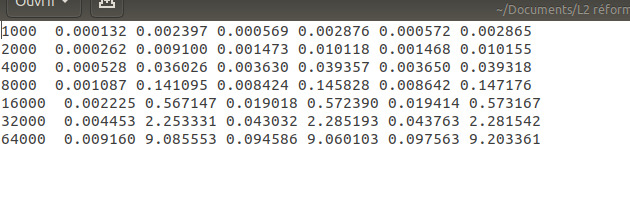
\includegraphics[scale=0.4]{images/resultat.jpeg}
\end{center}
\end{frame}
\section{Quelques graphiques}
\begin{frame}
\frametitle{Quelques Graphiques}
\begin{center}
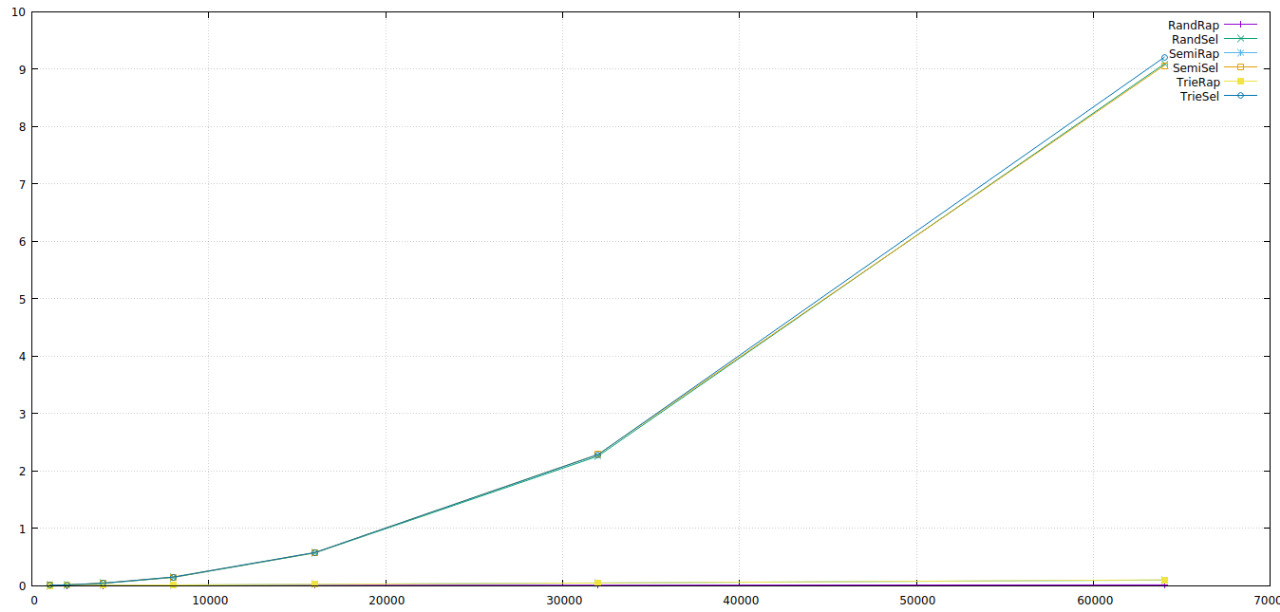
\includegraphics[scale=0.15]{images/graph1.jpeg}
\vspace{0.1cm}
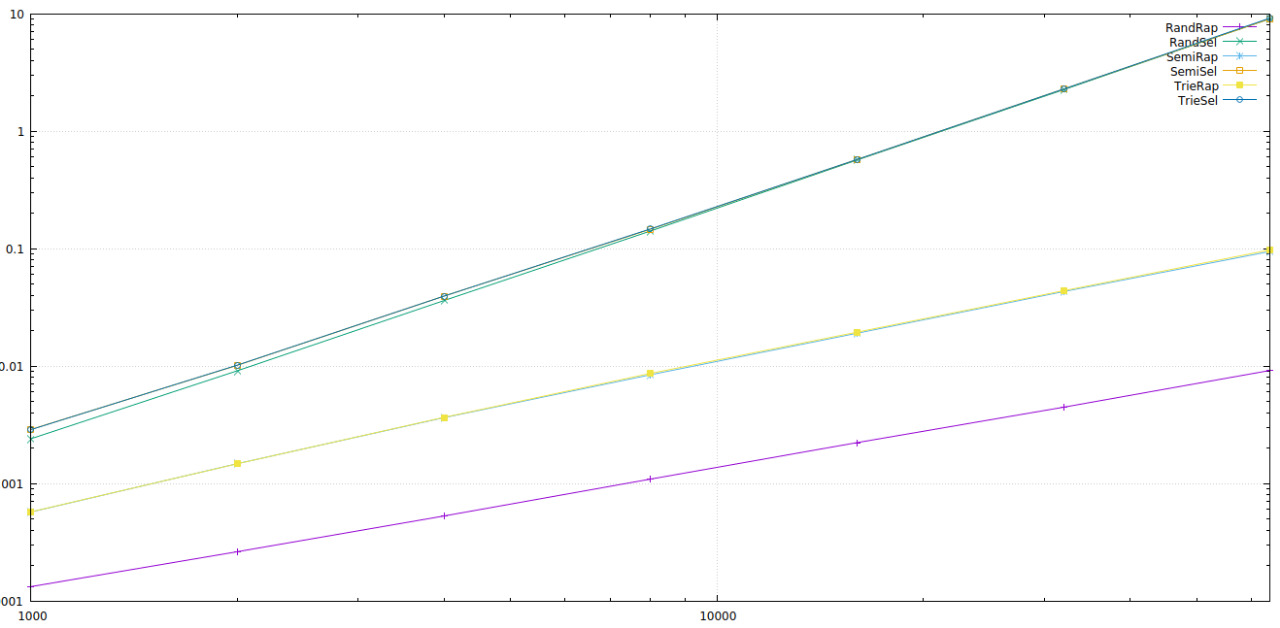
\includegraphics[scale=0.15]{images/graph2.jpeg}
\end{center}
\end{frame}
\section{Conclusion}
\begin{frame}
\frametitle{Conclusion}
Bien qu’il ne soit pas potentiellement réalisable d’évaluer avec exactitude la rapidité des deux modes de tris étudiés dans absolument tous les cas de figure, il en ressort néanmoins, à travers l’étude des différents graphs évalués en amont, que le Tri rapide reste dans la plupart des cas une méthode bien plus rapide que le Tri par sélection  \\
\end{frame}
\end{document}